\begin{titlepage}
    \section{Contexto do Sistema}
      Com o avanço das tecnologias de banco de dados e a ampla adoção de soluções baseadas em SQL e NoSQL, espera-se uma transição natural para formatos mais flexíveis e escaláveis. No entanto, muitos sistemas governamentais e corporativos ainda utilizam arquivos .DBF (dBase File) como meio principal para armazenamento e transferência de dados. Essa permanência se deve à forte dependência de sistemas legados, à complexidade da migração e à necessidade de interoperabilidade com aplicações antigas.
      Embora o formato .DBF seja uma tecnologia consolidada, sua utilização moderna apresenta desafios, principalmente na conversão e manipulação eficiente desses arquivos. A ausência de ferramentas atualizadas que permitam uma transição fluida para estruturas de dados contemporâneas impacta diretamente a eficiência dos sistemas que ainda dependem desse formato.
    \subsubsection{O que é um arquivo .DBF?}
    Criado na década de 1980 pelo software dBase, o .DBF foi amplamente adotado em aplicações que necessitavam de armazenamento tabular simples e acessível. Seu design permitiu que diversos sistemas gerenciassem registros estruturados de forma local, sem a necessidade de servidores de banco de dados.
    A compatibilidade do .DBF com tecnologias como FoxPro, Clipper, Visual dBase e xBase reforçou sua adoção em ambientes corporativos e governamentais. Sua estrutura de tabelas organizadas em colunas, associada à facilidade de acesso direto aos registros, tornou-o uma opção atrativa para sistemas de médio e grande porte durante o final do século XX.
    \subsubsection{Características do Formato .DBF}
    \begin{itemize}
        \item \textbf{Cabeçalho}: Define os campos da tabela (nome, tipo de dado, tamanho).
        \item \textbf{Registros}: Contêm os dados armazenados, com tamanho fixo por linha.
        \item \textbf{Marcação de exclusão}: Permite que registros sejam "deletados" sem removê-los fisicamente, o que acelera operações.
    \end{itemize}
    Essa arquitetura, embora eficiente para aplicações standalone, apresenta limitações significativas em operações de manipulação em larga escala, dificultando a integração com sistemas modernos que dependem de bancos de dados relacionais ou não relacionais.

    \subsubsection{Exemplos de Sistemas Governamentais que Utilizam .DBF}
    Apesar das limitações, o .DBF continua sendo um componente essencial em diversas infraestruturas governamentais brasileiras, como:
    \begin{itemize}
        \item \textbf{SINAN (Sistema de Informação de Agravos de Notificação)}: Utilizado pelo Ministério da Saúde do Brasil para armazenar informações sobre doenças e agravos de notificação compulsória.
        \item \textbf{SIA/SUS (Sistema de Informações Ambulatoriais do SUS)}: Responsável pelo processamento de atendimentos ambulatoriais em unidades de saúde pública.
        \item \textbf{SEFIP (Sistema Empresa de Recolhimento do FGTS e Informações à Previdência Social)} Utilizado para envio de dados de FGTS e Previdência Social.
        \item \textbf{SPED (Sistema Público de Escrituração Digital)}: Algumas aplicações dentro do SPED Fiscal ainda permitem exportações em .DBF.
        \item \textbf{Sistemas Cartorários e Notariais}: Muitos cartórios brasileiros utilizam .DBF para armazenar registros de imóveis, certidões e transações. Sistemas de Prefeituras e Estados – Diversos sistemas de arrecadação tributária, controle de IPTU, alvarás e cadastros imobiliários operam com .DBF.
    \end{itemize}
    A permanência desses sistemas reflete a necessidade de ferramentas que facilitem a interoperabilidade entre .DBF e outras estruturas de dados mais flexíveis, como JSON, CSV e bancos relacionais.
    \subsubsection{Por Que o Governo Brasileiro Ainda Utiliza .DBF?}
    A continuidade do uso do .DBF no Brasil não é apenas uma questão de preferência tecnológica, mas sim uma consequência de fatores estruturais, incluindo:
    \begin{itemize}
        \item \textbf{Histórico de uso e legado}:
              \subitem - Muitas aplicações desenvolvidas entre os anos 1980 e 2000 foram construídas utilizando dBase, Clipper, FoxPro, entre outras tecnologias baseadas em .DBF.
              \subitem - Esses sistemas continuam sendo utilizados, pois a migração para bancos modernos é custosa e complexa.
        \item \textbf{Facilidade de Integração}:
              \subitem - O formato .DBF é simples de manipular e pode ser lido por diversas linguagens de programação sem necessidade de drivers complexos.
              \subitem - O formato .DBF é simples de manipular e pode ser lido por diversas linguagens de programação sem necessidade de drivers complexos.
        \item \textbf{Baixo Custo e Independência de Banco de Dados}:
              \subitem - .DBF pode ser acessado sem um banco de dados SQL ou servidor dedicado, o que reduz os custos operacionais.
              \subitem - O governo brasileiro utiliza o formato .DBF em diversos sistemas para facilitar o armazenamento e a transmissão de dados entre diferentes órgãos e softwares.
    \end{itemize}

    Assim querendo resolver o problema de: Esses sistemas muitas vezes não possuem
    ferramentas modernas para manipulação de .DBF, tornando difícil a conversão
    para formatos mais flexíveis, como JSON e CSV. A ENVOLVE está propondo a a
    criação de uma biblioteca moderna e performática para conversão e manipulação
    de arquivos .DBF, utilizando Bun para maximizar a velocidade e eficiência na
    manipulação de arquivos binários. Diferente das soluções disponíveis, este
    sistema será modular e escalável, seguindo Domain-Driven Design (DDD) para
    garantir baixo acoplamento e facilidade de manutenção.

    \subsubsection{Motivação para o Uso de JavaScript/Bun}
    Embora linguagens como Go e Rust ofereçam alto desempenho, optamos por
    JavaScript/Bun devido a fatores críticos como ecossistema, suporte à web e
    acessibilidade para desenvolvedores. Além disso, consideramos Deno, mas optamos
    por Bun por razões específicas detalhadas a seguir.
    \begin{itemize}
        \item \textbf{Falta de Bibliotecas Atualizadas para .DBF em Node.js/Deno}:
              \subitem - \textbf{Node.js}: As bibliotecas existentes para manipulação de .DBF estão desatualizadas ou limitadas.
              \subitem - \textbf{Deno}: Embora existam bibliotecas como deno-dbf-file, elas ainda estão em estágios iniciais de desenvolvimento e podem não oferecer todas as funcionalidades necessárias.
        \item \textbf{Popularidade do JavaScript em APIs e Soluções Web}:
              \subitem - JavaScript é amplamente utilizado no desenvolvimento web, tornando a biblioteca mais acessível para a comunidade de desenvolvedores.
              \subitem - A ENVOLVE já possui experiência com JavaScript e TypeScript, o que acelera o desenvolvimento e a manutenção do sistema. 
        \item \textbf{Ecossistema de Módulos e Ferramentas}:
              \subitem - possui um ecossistema robusto com inúmeras bibliotecas e frameworks, facilitando a integração e expansão da funcionalidade.
              \subitem - Ferramentas como Bun permitem a criação de aplicações performáticas e escaláveis, garantindo alta eficiência no processamento de arquivos .DBF.
              \subitem - Bun oferece desempenho superior ao Node.js e comparável ao Deno, sendo adequado para operações de E/S intensivas.
              \subitem - A biblioteca será otimizada para manipulação de arquivos .DBF, garantindo alta velocidade e eficiência na conversão e leitura de dados.
        \item  \textbf{Manutenção e Facilidade de Distribuição}:
              \subitem - permite distribuição simplificada através do NPM, facilitando a instalação e atualização da biblioteca.
    \end{itemize}

    \subsubsection{Justificativa para a Escolha de Bun}
    \begin{itemize}
        \item Há uma lacuna no ecossistema JavaScript para bibliotecas modernas de
              manipulação de .DBF.
        \item JavaScript é amplamente utilizado, tornando a biblioteca mais acessível e
              incentivando a adoção.
        \item JavaScript possui um ecossistema rico que facilita a integração e expansão da
              funcionalidade.
        \item Bun oferece desempenho suficiente para as necessidades do projeto, equilibrando
              velocidade e facilidade de desenvolvimento.
        \item A distribuição via NPM/Bun simplifica a instalação e atualização da biblioteca.
        \item  Bun é mais rápido que Node.js e oferece desempenho comparável ao Deno.
        \item Essencial para manipulação eficiente de arquivos .DBF.
        \item oferece uma experiência de desenvolvimento simplificada, acelerando o processo
              de criação e manutenção da biblioteca.
        \item Desenvolvedores familiarizados com JavaScript podem adotar Bun rapidamente,
              reduzindo o tempo de adaptação.
    \end{itemize}

    \subsection{Arquitetura do Sistema}
    \textbf{Visão Geral da Arquitetura}:
    A biblioteca seguirá uma arquitetura modular, baseada em Domain-Driven Design (DDD) e organizada em três camadas principais:
    \begin{itemize}
        \item \textbf{Camada de Domínio (CORE DOMAIN) "core/"}: Contém as regras de negócio, garantindo a estrutura correta do .DBF.
        \item \textbf{Camada de Aplicação ((Application Layer) "application/")}: Orquestra os casos de uso e a conversão de formatos.
        \item \textbf{Camada de Infraestrutura (Infrastructure Layer): "infrastructure/"}: Responsável por persistência, manipulação de arquivos e parsers, mantendo-se desacoplada para permitir substituições futuras.
    \end{itemize}

    \begin{figure}[H]
        \centering
        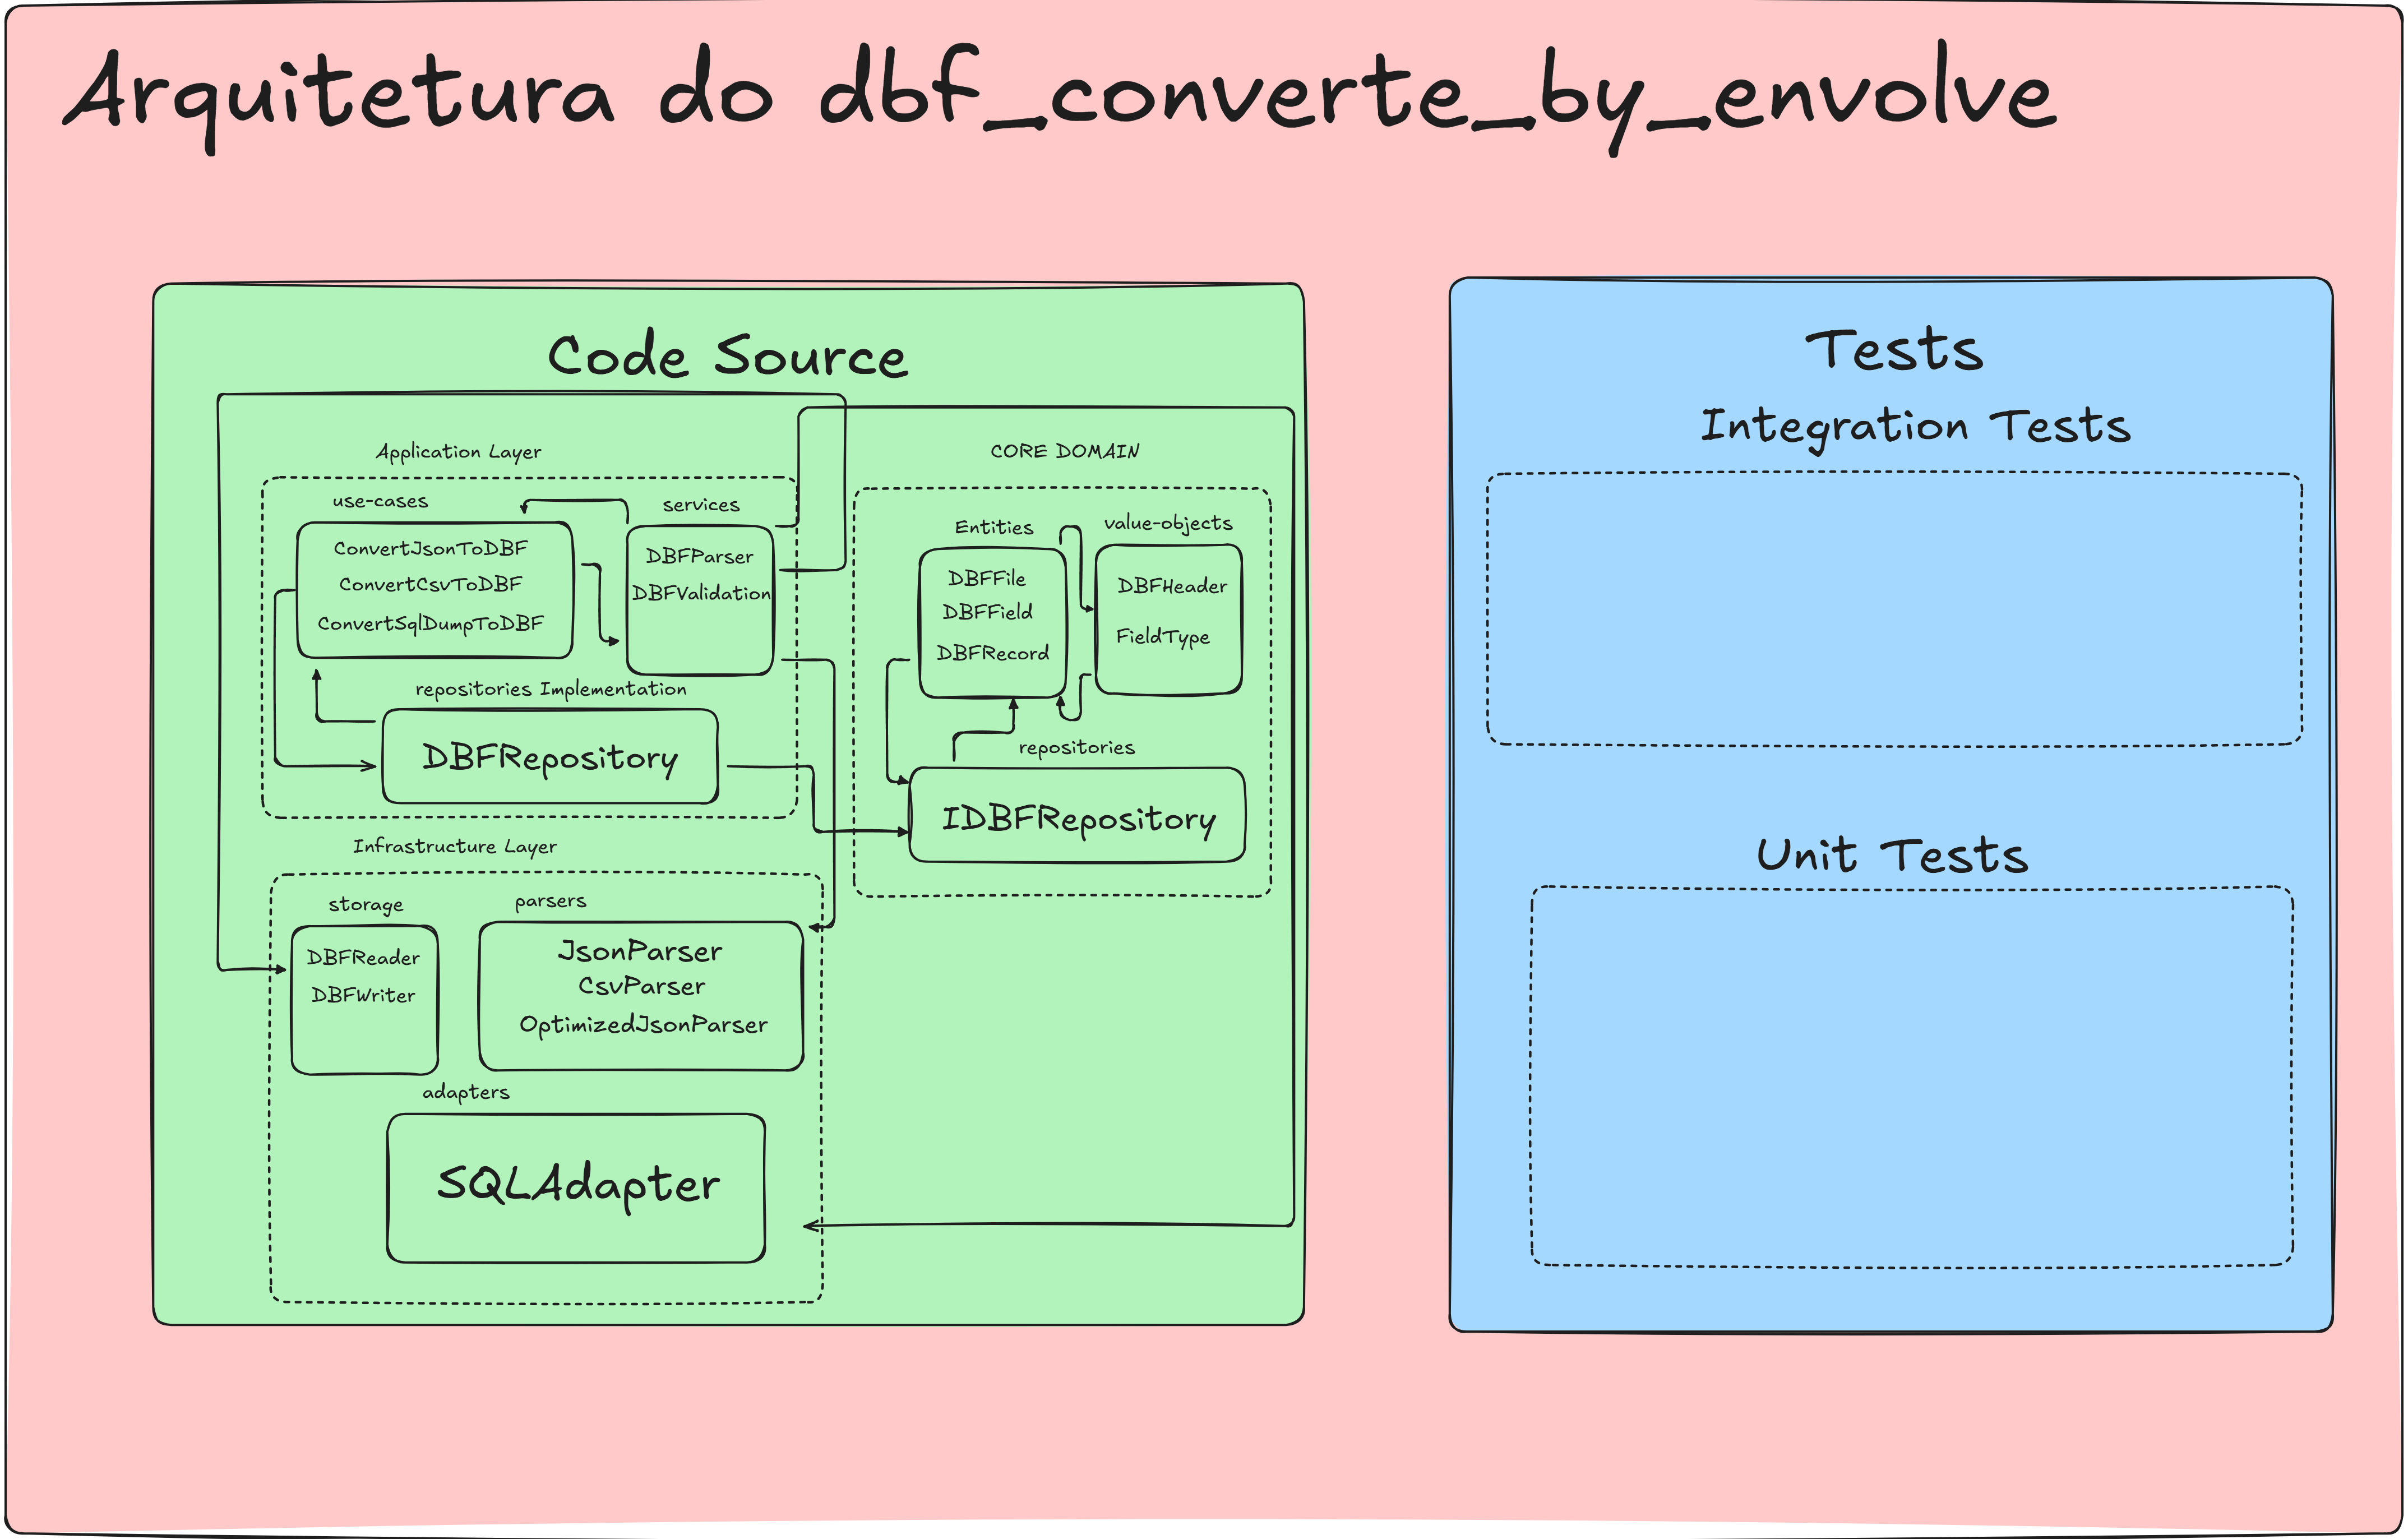
\includegraphics[width=0.8\textwidth]{image/dbf_converter_arquitetura.png}
        \caption{Arquitetura do Sistema}
        \label{fig:minha_imagem}
    \end{figure}

    \subsection{CORE DOMAIN - DBFStructure}
    O domínio `DBFStructure` é responsável por definir, validar e gerenciar
    arquivos no formato `.DBF`, um dos formatos de banco de dados mais utilizados
    historicamente. Apesar de ser um padrão antigo, ele ainda é amplamente adotado
    em sistemas governamentais, softwares contábeis e aplicações legadas devido à
    sua simplicidade, compatibilidade e estrutura binária eficiente. No entanto,
    essa mesma rigidez estrutural impõe desafios na manipulação desses arquivos,
    exigindo um modelo bem definido para garantir consistência, compatibilidade e
    confiabilidade ao armazenar e recuperar informações.

    O `DBFStructure` foi projetado para oferecer uma solução modular e extensível
    para manipulação de arquivos `.DBF`, permitindo que diferentes aplicações
    trabalhem com esses dados sem precisar lidar diretamente com a complexidade do
    formato. Esse domínio é responsável por definir a estrutura inicial dos
    arquivos, gerenciar a manipulação de registros e validar a integridade
    estrutural, garantindo que todas as operações respeitem as regras do `.DBF` e
    evitem corrupção dos dados.

    Para garantir a separação de responsabilidades, o `DBFStructure` foi organizado
    em \textbf{Bounded Contexts}, cada um com um papel específico na manipulação dos
    arquivos `.DBF`. Esses contextos garantem que operações distintas, como
    definição da estrutura, manipulação de registros e validação, sejam tratadas de
    forma isolada, minimizando dependências e permitindo evolução independente de
    cada módulo.

    Os principais `Bounded Contexts` do domínio `DBFStructure` são:

    \begin{itemize}
        \item \textbf{DBFFileDefinition}: Responsável pela criação e definição da estrutura do `.DBF`, incluindo seu cabeçalho (`DBFHeader`), campos (`DBFField`) e regras de estruturação. Esse contexto também gerencia a adição, alteração e remoção de campos dentro do arquivo, garantindo que qualquer modificação estrutural seja validada antes de ser aplicada. \textbf{Qualquer modificação na estrutura (`DBFField`) resultará na exclusão automática de todos os registros (`DBFRecord`) existentes no arquivo.}

        \item \textbf{DBFRecordManagement}: Responsável pelo gerenciamento dos registros (`DBFRecord`) dentro de um arquivo `.DBF`, incluindo operações de inserção, remoção e edição de registros. \textbf{Esse contexto depende da estrutura definida pelo `DBFFileDefinition` e só pode operar sobre arquivos `.DBF` previamente validados.}

        \item \textbf{DBFValidation}: Responsável pela validação estrutural e de dados dos arquivos `.DBF`, garantindo que qualquer modificação realizada dentro do `DBFFileDefinition` ou `DBFRecordManagement` esteja dentro das regras do formato `.DBF`, assegurando consistência e integridade.

        \item \textbf{DBFExport}: Responsável pela conversão da estrutura interna do `.DBF` para um arquivo binário `.DBF` válido, garantindo que os dados e a estrutura sejam corretamente escritos em disco, permitindo que o arquivo seja utilizado por sistemas externos.
    \end{itemize}

    A modularidade do `DBFStructure` permite que cada um desses contextos evolua
    independentemente, possibilitando melhorias contínuas sem impactar
    funcionalidades já existentes. Além disso, essa abordagem facilita a integração
    com infraestruturas externas, como conversores de formatos (`JSON`, `CSV`, `SQL
    Dump`), sistemas de banco de dados relacionais e APIs que precisem manipular
    `.DBF`.

    O diferencial do `DBFStructure` não está apenas em fornecer um modelo robusto
    para lidar com `.DBF`, mas também em permitir sua evolução gradual. O design
    modular do domínio possibilita suporte a novos formatos, versões mais recentes
    do `.DBF`, e melhorias na validação, tornando os arquivos `.DBF` mais
    acessíveis para integração com sistemas modernos sem perda de confiabilidade ou
    compatibilidade.

    \subsubsection{Objetivos}
    \begin{itemize}
        \item Definir a Estrutura de um Arquivo `.DBF`, garantindo que cabeçalhos, campos e
              registros sigam as regras do formato.
        \item Gerenciar Registros (`DBFRecord`) do `.DBF`, permitindo inserção, edição e
              remoção sem comprometer a estrutura.
        \item Modificar a estrutura do `.DBF` (`DBFField`), permitindo a adição e remoção de
              colunas. \textbf{Qualquer alteração na estrutura resulta na exclusão automática de
              todos os registros (`DBFRecord`).}
        \item Validar a Estrutura do `.DBF` para garantir integridade e compatibilidade com
              sistemas que utilizam esse formato.
        \item Assegurar Consistência e Compatibilidade do Arquivo, respeitando os limites de
              tamanho, alinhamento e regras de versionamento.
        \item Facilitar a Integração com Outras Tecnologias, permitindo exportação e
              conversão para formatos modernos.
    \end{itemize}

    \subsubsection{Futuros Objetivos}
    \begin{itemize}
        \item Suporte a Novos Formatos de Exportação (`XML`, `Parquet`, `YAML`).
        \item Suporte a Campos do Tipo Memo (`M`), utilizados em versões mais recentes do
              `.DBF` para armazenamento de textos longos.
        \item Suporte a Diferentes Versões do `.DBF` (dBase IV (0x04), dBase V (0x05), FoxPro
              (0x30)).
        \item Melhorias na Validação e Correção Automática de Estruturas `.DBF` corrompidas.
        \item Integração com Banco de Dados Relacionais, permitindo conversões diretas entre
              `.DBF` e `PostgreSQL`, `MySQL`, `SQLite` e outros.
    \end{itemize}

    \begin{titlepage}
    \subsection{Bounded Context}

    \begin{enumerate}
        \item   DBFFileDefinition: Define a estrutura inicial do arquivo .DBF, incluindo o
              cabeçalho (DBFHeader) e os campos (DBFField). Este contexto é responsável pela
              criação da estrutura base do arquivo e não gerencia a adição, remoção ou
              alteração de campos.
        \item   DBFFieldManagement: Gerencia a adição, alteração e remoção de campos (DBFField)
              dentro do arquivo .DBF. Assegura que qualquer modificação estrutural seja
              validada e aplicada corretamente. Qualquer modificação na estrutura de campos
              resulta na remoção lógica dos registros (DBFRecord).
        \item   DBFRecordManagement: Gerencia a manipulação dos registros (DBFRecord) dentro do
              arquivo .DBF, permitindo a inserção, edição, remoção lógica e recuperação de
              registros. Opera sobre arquivos .DBF com estrutura previamente validada.
        \item   DBFValidation: Valida a estrutura e os registros do .DBF. Garante que qualquer
              modificação nos contextos DBFFileDefinition, DBFFieldManagement e
              DBFRecordManagement esteja em conformidade com as regras do formato .DBF.
        \item   DBFExport: Converte a estrutura interna do .DBF para um arquivo binário .DBF
              válido e o armazena, garantindo a correta escrita dos dados e da estrutura para
              uso externo.
        \item   DBFImport: Importa dados de fontes externas (e.g., CSV, JSON) para a estrutura
              interna do .DBF. Garante que os dados importados estejam em conformidade com a
              estrutura definida e cria os registros (DBFRecord) correspondentes.
    \end{enumerate}

    \subsection{Definição do BOUNDED CONTEXT: DBFFileDefinition}
O DBFFileDefinition é o núcleo responsável por estabelecer a estrutura inicial de um arquivo .DBF. Ele assegura que a estrutura base seja válida e compatível com as regras do formato .DBF. Esse contexto gerencia a criação da "casca" do arquivo, preparando-o para operações futuras, como inserção de registros (DBFRecord) ou exportação (DBFExport).
Os arquivos .DBF seguem um formato binário rígido, onde cada componente: \\
 - DBFHeader (cabeçalho) \\
 - DBFField (campos) \\
 - DBFRecord (registros) \\
precisa estar corretamente alinhado e estruturado para garantir compatibilidade com sistemas que processam esse tipo de dado. Um erro na definição estrutural pode tornar o arquivo ilegível para outros sistemas, tornando a configuração correta da estrutura um aspecto crítico.
Esse contexto atua diretamente na criação da estrutura inicial de um .DBF. Ele define regras para nomes de campos, tipos de dados, tamanho dos registros e alinhamento da memória, garantindo que a estrutura seja construída corretamente desde o início. É importante ressaltar que, nesse estágio, as listas de campos (List<DBFField>) e registros (List<DBFRecord>) são inicializadas vazias. \\

\begin{bclogo}[logo=\bcattention, couleurBarre=red, noborder=true, 
    couleur=LightSalmon]{Important!}
    \begin{itemize}
        \item O DBFFileDefinition é responsável pela criação da "casca" inicial do arquivo .DBF.
        \item Neste contexto, as listas de campos (List<DBFField>) \\ e registros (List<DBFRecord>) são inicializadas vazias.
        \item A validação completa do arquivo .DBF só deve ocorrer após a adição de dados e é responsabilidade de outro contexto (DBFValidation).
    \end{itemize}
\end{bclogo}

O DBFFileDefinition será modelado como um agregado (Aggregate Root), onde o DBFFile atuará como a raiz do agregado. Esse agregado encapsula toda a estrutura inicial do .DBF.
O DBFFile conterá as seguintes estruturas: 
\begin{itemize}
    \item DBFHeader: Metadados do .DBF, incluindo versão, data de modificação, contagem de registros e deslocamento do primeiro registro. \\
    \item List<DBFField>: Lista de campos (DBFField) que definem a estrutura do .DBF, incluindo nome, tipo de dado e tamanho. 
    \item List<DBFRecord>: Lista de registros (DBFRecord), que é inicializada vazia. 
\end{itemize}

\textbf{Esse agregado garantirá que:}
\begin{itemize}
    \item A estrutura inicial do .DBF seja consistente e válida.
    \item O DBFFileDefinition não gerencia a adição, remoção ou alteração de campos, nem a manipulação de registros. Essas são responsabilidades de outros Bounded Contexts.
\end{itemize}

\subsection{Organização do DBFFileDefinition}

O DBFFileDefinition é responsável pela criação da estrutura inicial do .DBF, garantindo que ele seja construído de maneira válida e coerente. Ele tem como foco exclusivo a definição da "casca" do arquivo, ou seja, a estrutura base, preparando-o para receber dados e ser utilizado por outros contextos. Este contexto não gerencia a modificação de campos (DBFField) ou a manipulação de registros (DBFRecord).\\

\textbf{Responsabilidades Exclusivas:} 

\begin{enumerate}
    \item O DBFFileDefinition não gerencia a adição, remoção ou alteração de campos (DBFField).
    \item O DBFFileDefinition não gerencia a manipulação de registros (DBFRecord).
    \item Essas responsabilidades são delegadas aos Bounded Contexts DBFFieldManagement e DBFRecordManagement, respectivamente.
\end{enumerate}

\subsection{Como Esse Contexto Será Implementado?}
O DBFFileDefinition será modelado como um agregado (Aggregate Root), onde o DBFFile atuará como a raiz do agregado. Esse agregado encapsula a estrutura inicial do .DBF, representando a "casca" do arquivo.
\subsubsection{Tarefas Principais do DBFFileDefinition}
O DBFFileDefinition tem como tarefas principais a criação da estrutura inicial do .DBF e a preparação para sua utilização por outros contextos. \\\\
\textbf{Gerenciamento da Estrutura Inicial:} \\\\
- Criar um novo arquivo .DBF, definindo o cabeçalho (DBFHeader) e inicializando a lista de campos (List<DBFField>) e a lista de registros (List<DBFRecord>) como vazias. \\
- Garantir que o tamanho do cabeçalho seja calculado corretamente. \\
- Determinar a posição (offset) do primeiro registro dentro do arquivo. \\\\
\textbf{Preparação para Outros Contextos:} \\\\
- Fornecer a "casca" do .DBF pronta para ser populada com dados e validada (DBFValidation). \\
- Garantir que a estrutura inicial definida seja compatível com a exportação (DBFExport). \\

\subsubsection{Tipos de dados do DBFFileDefinition}
\textbf{Esta seção detalha os tipos de dados utilizados no contexto DBFFileDefinition, suas propriedades e as regras de negócio associadas}

\subsubsection{Informações gerais do DBFFile}
\begin{itemize}
    \item \textbf{Nome do dado}: \textit{\textbf{DBFFile}}
    \item \textbf{Tipo do dado}: \textit{\textbf{Aggregate Root}}
    \item \textbf{Descrição do dado}: O \textit{\textbf{DBFFile}} é a raiz do agregado e centraliza todas as regras de criação e manipulação da estrutura do \textit{\textbf{.dbf}}. Ele encapsula o cabeçalho: \textit{\textbf{DBFHeader}}, a lista de campos:\textit{\textbf{List<DBFField>}} e os registros:\textit{\textbf{List<DBFRecord>}}, garantindo que nenhuma modificação ocorra de maneira inconsistente.
\end{itemize}


\begin{table}[H]
    \centering
    \textbf{Atributos do Aggregate Root DBFFile}
    \begin{tabular}{|p{0.2\textwidth} | p{0.3\textwidth} | p{0.5\textwidth}|}
        \hline
        \textbf{Atributo} & \textbf{Tipo} & \textbf{Descrição} \\
        \hline
        name & string & Nome do arquivo .DBF. \\
        \hline
        header & DBFHeader & Metadados do .DBF (versão, data, quantidade de registros). \\
        \hline
        fields & List<DBFField> & Lista de colunas (campos da tabela). \\
        \hline
        records & List<DBFRecord> & Lista de registros armazenados dentro do .DBF. \\
        \hline
        recordSize & number & Define o tamanho dos Registros deste dbf, sendo calculado pela soma em bytes dos CAMPOS do arquivo \\
        \hline
    \end{tabular}
    \caption{Atributos do DBFFile e suas descrições}
    \label{tab:tabela_atributos_dbffile}
\end{table}

\subsubsection{Metodos que estão dentro do DBFFile}
\begin{itemize}
    \item \textbf{create}: Método responsável por criar a instancia do DBFFile, A implementação não amarra como será feita, caso queira usar um factory ou um builder, a seu criterio. Sempre uma nova instancia for criada, lembre-se que os campos fields e records devem ser listas vazias. O DBFHeader não pode está vazia.
    \item \textbf{calculateRecordSize}: Método responsável por calcular o tamanho da soma de todos os campos: \textit{\textbf{DBFField}} em bytes.
    \item \textbf{validateHeaderSize}: Método responsável por validar o tamanho do cabeçalho, o tamanho do cabeçalho deve ser múltiplo de 32 bytes. Ou seja, caso o tamanho do cabeçalho em bytes for um numero que não é multiplo de 32, o sistema tem que adicionar a quantidade de bytes com zeros até que o tamanho seja múltiplo de 32.
\end{itemize}

\subsubsection{Informações Gerais do DBFField}
\textbf{Nome do dado}: \textit{\textbf{DBFField}} \\  
\textbf{Tipo do dado}: Entidade \\  
\textbf{Descrição do dado}: Cada DBFField representa um campo dentro do \textit{\textbf{.bdf}}, definindo nome, tipo, tamanho e alinhamento dos dados armazenados. \\  

\begin{table}[H]
    \centering
    \textbf{Atributos da entidade do DBFField}
    \begin{tabular}{|p{0.2\textwidth} | p{0.3\textwidth} | p{0.5\textwidth}|}
        \hline
        \textbf{Atributo} & \textbf{Tipo} & \textbf{Descrição} \\
        \hline
        name & string & Nome do campo da tabela \\
        \hline
        type & enum &  Um enumerador com os valores permitidos: ver os valores na tabela do enum abaixo. \\
        \hline
        size & number  & Tamanho do campo em bytes. \\
        \hline
        decimal & number  & Aqui fica qual o número de casas decimais que será colocado, quando os registros forem escritos. Exemplo: Caso você queira o numero 12 e coloque no tamanho do campo sendo 2, está tudo bem, pois o binario será: 0x31 0x32. Porém se for colocado no tamanho do campo 5 bytes e só dois decimais, ai a representação do numero será: 0x31 0x32 0x2E 0x30 0x30, Pois obrigatoriamente quando é colocado só 2 decimais o resto será flutuante, então será 1 caracter para o ponto e outros dois para zeros \\
        \hline
    \end{tabular}
    \caption{Atributos do DBFField e suas descrições}
    \label{tab:tabela_atributos_dbffield}
\end{table}

\begin{table}[H]
    \centering
    \textbf{Enumerator do campo type do DBFField}
    \begin{tabular}{|p{0.2\textwidth} | p{0.3\textwidth} | p{0.5\textwidth}|}
        \hline
        \textbf{Atributo} & \textbf{Tipo} & \textbf{Descrição} \\
        \hline
        C & Character & É um tipo que aceita textos, porém com o tamanho máximo sendo de 10 bytes \\
        \hline
        N & Numeric &  É um tipo que aceita numeros em geral, tanto decimais, quanto inteiros, porém com um tamanho máximo de 19 bytes \\
        \hline
        F & Float  & É um tipo que aceita as mesmas regras do Numeric, porém é para numeros flutuantes com menor precisão \\
        \hline
        L & Logical  & Booleano (T ou F, para verdadeiro ou falso). Sendo seu maximo 1 byte \\
        \hline
        D & Date  & Data no formato YYYYMMDD (8 caracteres). \\
        \hline
    \end{tabular}
    \caption{Todos os valores possiveis que podem ser escolhidos para o campo type do \textit{\textbf{DBFField}}}
    \label{tab:tabela_enumeracao_atributo_type}
\end{table}

\subsubsection{Metodos que estão dentro do DBFFile}
\begin{itemize}
    \item \textbf{create}: Método responsável por criar a instancia do \textit{\textbf{DBFField}}, Ou seja ele cria um BDFFiel válido para ser colocado dentro da lista de \textit{\textbf{DBFField}}.
    \item \textbf{validateNameField}: Método responsável por validar o nome do campo, o nome do campo não pode ser vazio, e nem pode ter mais de 10 caracteres. 
    \item \textbf{calculateSize}: Calcula o tamanho do campo em bytes, baseado no tipo de dado. Caso não contenha já registros, se sim pegue o maior registro deste campo e coloque como o tamanho.
\end{itemize}






\subsubsection{Informações Gerais do DBFHeader}
\textbf{Nome do dado}: \textit{\textbf{DBFHeader}} \\  
\textbf{Tipo do dado}: Entidade \\  
\textbf{Descrição do dado}: Cada DBFField representa um campo dentro do \textit{\textbf{.bdf}}, definindo nome, tipo, tamanho e alinhamento dos dados armazenados. \\  

\subsubsection{Atributos do DBFHeader}  
\textbf{version: enum} - Versão do `.DBF`. (`0x03` para `dBase III`). \\  
\textbf{lastUpdated: Date} - Data da última modificação do arquivo. \\  
\textbf{recordCount: number} - Número total de registros armazenados (`DBFRecord`). \\  
\textbf{firstRecordOffset: number} - Offset (posição em bytes) do primeiro registro dentro do arquivo. \\  

\subsubsection{Regras de negócio do DBFHeader}
\begin{enumerate}
    \item O offset do primeiro registro (`firstRecordOffset`) deve ser sempre múltiplo de 32 bytes.
    \item A versão do `.DBF` deve ser compatível (`0x03` para `dBase III`).
    \item O número de registros (`recordCount`) deve ser atualizado corretamente sempre que um registro (`DBFRecord`) for adicionado ou removido.
\end{enumerate}


\subsection{Diagrama de Classes do DBFFileDefinition}
\begin{figure}[H]
    \centering
    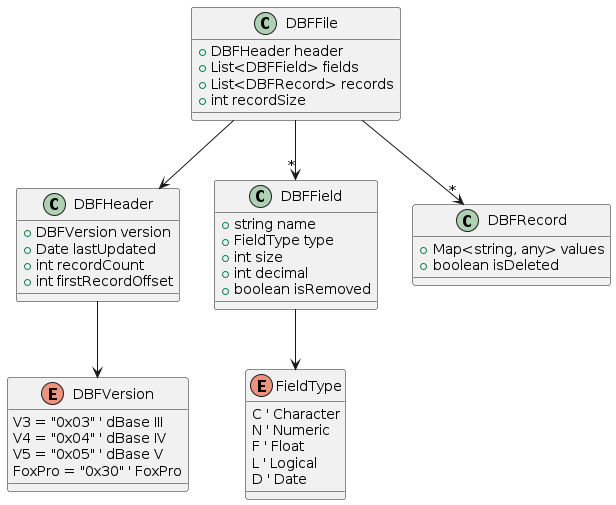
\includegraphics[width=1\textwidth]{image/uml_DBFESTRUCTURE.png}
    \caption{Diagrama de Classes do Bounded Context: DBFFileDefinition}
\end{figure}

\subsection{BDD do caso de uso: CreateDBFFileBaseV3}
\subsubsection{Feature: Criar um objeto DBFFile válido}
Como um usuário ou sistema \\
Quero criar um objeto \textbf{DBFFile} contendo: \\
- \textbf{DBFHeader}\\
- \textbf{List<DBFField>} \\
- \textbf{List<DBFRecord>}\\
inicializados corretamente Para que ele possa ser utilizado posteriormente por outros casos de uso \\

\subsubsection{Background}
\textbf{Given} que \textbf{DBFFile} representa um arquivo `.DBF` na memória \\
\textbf{And} \textbf{DBFFile} deve ser criado apenas com: \\
- \textbf{DBFHeader} \\
- \textbf{List<DBFField>}\\
- \textbf{List<DBFRecord>}\\
todos inicializados corretamente

\subsubsection{Scenario: Criar um objeto DBFFile com campos e registros válidos}
\textbf{Given} que o sistema inicia a criação de um \textbf{DBFFile} \\
\textbf{When} o sistema cria um \textbf{DBFHeader} \\
\textbf{And} o \textbf{DBFHeader} contém a versão padrão do `.DBF` (`0x03`) \\
\textbf{And} o \textbf{DBFHeader} contém a data atual como última modificação \\
\textbf{And} o \textbf{DBFHeader} tem o número total de registros inicializado como zero \\
\textbf{And} o \textbf{DBFHeader} calcula a posição inicial onde os registros serão armazenados \\
\textbf{And} o sistema inicializa uma \textbf{List<DBFField>} vazia \\
\textbf{And} o sistema inicializa uma \textbf{List<DBFRecord>} vazia \\
\textbf{Then} o sistema associa o \textbf{DBFHeader}, \textbf{List<DBFField>} e \textbf{List<DBFRecord>} ao \textbf{DBFFile} \\
\textbf{And} o sistema retorna um \textbf{DBFFile} pronto para ser manipulado \\

\subsubsection{Scenario: Criar um DBFFile sem registros iniciais}
\textbf{Given} que o sistema inicia a criação de um \textbf{DBFFile} \\
\textbf{When} o sistema cria um \textbf{DBFHeader} \\
\textbf{And} o sistema inicializa uma \textbf{List<DBFField>} vazia \\
\textbf{And} a \textbf{List<DBFRecord>} está vazia, pois não há registros no momento da criação \\
\textbf{Then} o sistema retorna um \textbf{DBFFile} válido contendo apenas cabeçalho e campos \\

\subsubsection{Scenario: Falha ao criar o DBFHeader}
\textbf{Given} que ocorreu um erro ao criar o \textbf{DBFHeader} \\
\textbf{When} o sistema tenta associar o \textbf{DBFHeader} ao \textbf{DBFFile} \\
\textbf{Then} o sistema deve lançar um erro \textbf{"Erro: Falha ao criar o cabeçalho do DBF"} \\
\textbf{And} o sistema não deve criar um \textbf{DBFFile} \\

\subsubsection{Scenario: Falha ao inicializar a lista de campos (`DBFField`)}
\textbf{Given} que ocorreu um erro ao criar a \textbf{List<DBFField>} vazia \\
\textbf{When} o sistema tenta associar a lista de campos ao \textbf{DBFFile} \\
\textbf{Then} o sistema deve lançar um erro \textbf{"Erro: A lista de campos deve ser inicializada vazia"} \\
\textbf{And} o sistema não deve criar um \textbf{DBFFile} \\

\subsubsection{Scenario: Falha ao inicializar a lista de registros (`DBFRecord`)}
\textbf{Given} que ocorreu um erro ao criar a \textbf{List<DBFRecord>} vazia \\
\textbf{When} o sistema tenta associar a lista de registros ao \textbf{DBFFile} \\
\textbf{Then} o sistema deve lançar um erro \textbf{"Erro: A lista de registros deve ser inicializada vazia"} \\
\textbf{And} o sistema não deve criar um \textbf{DBFFile} \\

\subsubsection{Scenario: Falha ao definir a versão do `.DBF`}
\textbf{Given} que o sistema inicia a criação de um \textbf{DBFFile} \\
\textbf{When} o sistema cria um \textbf{DBFHeader} \\
\textbf{And} a versão do `.DBF` não pode ser definida corretamente \\
\textbf{Then} o sistema deve lançar um erro \textbf{"Erro: Versão do `.DBF` inválida"} \\
\textbf{And} o sistema não deve criar um \textbf{DBFFile} \\

\subsubsection{Scenario: Falha ao definir a data da última modificação}
\textbf{Given} que o sistema inicia a criação de um \textbf{DBFFile} \\
\textbf{When} o sistema cria um \textbf{DBFHeader} \\
\textbf{And} ocorre um erro ao definir a data da última modificação \\
\textbf{Then} o sistema deve lançar um erro \textbf{"Erro: Data de modificação inválida"} \\
\textbf{And} o sistema não deve criar um \textbf{DBFFile} \\

\subsubsection{Scenario: Falha ao calcular o offset do primeiro registro}
\textbf{Given} que o sistema inicia a criação de um \textbf{DBFFile} \\
\textbf{When} o sistema cria um \textbf{DBFHeader} \\
\textbf{And} ocorre um erro ao calcular a posição inicial do primeiro registro \\
\textbf{Then} o sistema deve lançar um erro \textbf{"Erro: Falha ao calcular o offset do primeiro registro"} \\
\textbf{And} o sistema não deve criar um \textbf{DBFFile} \\


    \subsection{Definição do BOUNDED CONTEXT: DBFFieldManagement}
O \textbf{DBFFieldManagement} é responsável por gerenciar a estrutura dos campos (\textbf{DBFField}) dentro de um arquivo \textbf{.DBF}, permitindo \textbf{adição, modificação e remoção} de campos.

Os campos (\textbf{DBFField}) definem a estrutura do \textbf{.DBF}, ou seja, quais informações podem ser armazenadas nos registros (\textbf{DBFRecord}). Como o formato \textbf{.DBF} possui alinhamento fixo, \textbf{qualquer modificação nos campos exige a remoção de todos os registros (\textbf{DBFRecord}) existentes}, pois os dados podem ficar desalinhados e ilegíveis para outros sistemas.

\textbf{Esse contexto não gerencia registros (\textbf{DBFRecord})}, pois essa responsabilidade pertence ao \textbf{DBFRecordManagement}.

\subsection{Como Esse Contexto Será Implementado?}
O \textbf{DBFFieldManagement} será implementado como um conjunto de operações dentro do \textbf{DBFFile} (Aggregate Root). Ele permitirá modificar a estrutura dos campos (\textbf{DBFField}), garantindo que as mudanças respeitem as regras do \textbf{.DBF} e que os registros (\textbf{DBFRecord}) sejam excluídos automaticamente quando necessário.

\textbf{IMPORTANTE:} 
\begin{itemize}
    \item Qualquer \textbf{adição, modificação ou remoção de um DBFField} exige a \textbf{recriação da estrutura do .DBF}, pois os registros (\textbf{DBFRecord}) dependem diretamente dos campos.
    \item Após qualquer alteração estrutural, \textbf{todos os registros (\textbf{DBFRecord}) serão apagados automaticamente} para evitar inconsistências.
\end{itemize}

\subsection{Responsabilidades do DBFFieldManagement}
\begin{itemize}
    \item Adicionar um novo campo (\textbf{DBFField}) sem comprometer a estrutura do \textbf{.DBF}.
    \item Modificar um campo (\textbf{DBFField}) garantindo que a alteração respeite as regras do formato.
    \item Remover um campo (\textbf{DBFField}) e garantir que a estrutura permaneça válida.
    \item Assegurar que todas as modificações passem por validação (\textbf{DBFValidation}) antes de serem aplicadas.
    \item Atualizar metadados do \textbf{DBFHeader} (ex: \textbf{recordCount}) para refletir mudanças na estrutura.
    \item Garantir que qualquer modificação nos campos (\textbf{DBFField}) resulte na remoção automática dos registros (\textbf{DBFRecord}).
\end{itemize}

\subsection{Tipos de Dados no DBFFieldManagement}
O \textbf{DBFFieldManagement} lida diretamente com os seguintes componentes:

\subsubsection{DBFFile (Aggregate Root)}
\textbf{Descrição:} O \textbf{DBFFile} encapsula toda a estrutura do \textbf{.DBF}, incluindo os campos (\textbf{List<DBFField>}) e registros (\textbf{List<DBFRecord>}).

\begin{table}[h]
    \centering
    \begin{tabular}{|l|l|p{10cm}|}
        \hline
        \textbf{Atributo} & \textbf{Tipo} & \textbf{Descrição} \\ \hline
        \textbf{header} & DBFHeader & Contém metadados do \textbf{.DBF} (versão, data, contagem de registros). \\ \hline
        \textbf{fields} & List<DBFField> & Contém todos os campos do \textbf{.DBF}. \\ \hline
        \textbf{records} & List<DBFRecord> & Contém todos os registros armazenados. \\ \hline
        \textbf{recordSize} & number & Define o tamanho fixo de cada registro. \\ \hline
    \end{tabular}
\end{table}

\textbf{Regras de Negócio:}
\begin{enumerate}
    \item O \textbf{.DBF} deve ter pelo menos um \textbf{DBFField} para ser válido.
    \item Qualquer alteração em \textbf{DBFField} deve apagar todos os \textbf{DBFRecord} para evitar registros desalinhados.
    \item O \textbf{recordSize} deve ser recalculado sempre que um campo for adicionado, alterado ou removido.
\end{enumerate}

\subsubsection{DBFField}
\textbf{Descrição:} Cada \textbf{DBFField} representa uma coluna dentro do \textbf{.DBF}, definindo o nome, tipo, tamanho e alinhamento dos dados.

\begin{table}[h]
    \centering
    \begin{tabular}{|l|l|p{10cm}|}
        \hline
        \textbf{Atributo} & \textbf{Tipo} & \textbf{Descrição} \\ \hline
        \textbf{name} & string & Nome do campo (máx. 10 caracteres). \\ \hline
        \textbf{type} & enum & Define o tipo de dado armazenado. \\ \hline
        \textbf{size} & number & Tamanho do campo em bytes. \\ \hline
        \textbf{decimal} & number & Número de casas decimais (apenas para \textbf{N}). \\ \hline
        \textbf{isRemoved} & boolean & Indica se o campo foi marcado como "removido". \\ \hline
    \end{tabular}
\end{table}

\textbf{Regras de Negócio:}
\begin{enumerate}
    \item O nome do campo não pode exceder 10 caracteres.
    \item O tipo do campo deve ser válido (\textbf{C, N, F, L, D}).
    \item Se o campo for do tipo \textbf{Numérico (N)}, deve validar casas decimais (mín. 1, máx. 19 bytes).
    \item Se um campo for removido (\textbf{isRemoved}), ele não pode mais ser usado em novos registros.
\end{enumerate}

\subsection{Relação do DBFFieldManagement com Outros Contextos}

\subsubsection{DBFFileDefinition}
\textbf{Tipo de Relação:} \textbf{Shared Kernel} \\
\textbf{Descrição:} O \textbf{DBFFileDefinition} define a estrutura inicial do \textbf{.DBF}, enquanto o \textbf{DBFFieldManagement} permite modificá-la. Como ambos compartilham o mesmo \textbf{DBFFile}, mudanças devem ser feitas com \textbf{validação rigorosa}.

\subsubsection{DBFRecordManagement}
\textbf{Tipo de Relação:} \textbf{Customer/Supplier} \\
\textbf{Descrição:} Como os registros (\textbf{DBFRecord}) dependem dos campos (\textbf{DBFField}), qualquer modificação estrutural exige que todos os registros sejam apagados.

\subsubsection{DBFValidation}
\textbf{Tipo de Relação:} \textbf{Open-Host Service} \\
\textbf{Descrição:} Sempre que um campo (\textbf{DBFField}) for \textbf{adicionado, alterado ou removido}, o \textbf{DBFValidation} deve garantir que a estrutura do \textbf{.DBF} permaneça válida.

\subsubsection{DBFExport}
\textbf{Tipo de Relação:} \textbf{Published Language} \\
\textbf{Descrição:} O \textbf{DBFFieldManagement} define a estrutura do \textbf{.DBF}, garantindo que ele possa ser corretamente exportado pelo \textbf{DBFExport}.

\subsection{Conclusão}
O \textbf{DBFFieldManagement} desempenha um papel crucial dentro do \textbf{DBFStructure}, pois permite modificar a estrutura do \textbf{.DBF} sem comprometer sua integridade. Ele \textbf{não gerencia registros (\textbf{DBFRecord})}, mas garante que qualquer mudança nos campos (\textbf{DBFField}) seja segura e validada.

\subsubsection{Scenario: Adicionar um novo campo (`DBFField`) ao `.DBF`}
\textbf{Given} que o sistema possui um `DBFFile` válido com uma `List<DBFField>` existente \\
\textbf{When} o usuário solicita a adição de um novo `DBFField` \\
\textbf{Then} o sistema deve validar se o nome do campo não excede 10 caracteres \\
\textbf{And} o sistema deve validar se o tipo (`type`) do campo pertence ao conjunto permitido `{C, N, F, L, D}` \\
\textbf{And} o sistema deve validar que o nome do campo não está duplicado na `List<DBFField>` \\
\textbf{And} o sistema adiciona o novo `DBFField` à `List<DBFField>` \\
\textbf{And} o sistema remove todos os registros (`DBFRecord`) do `DBFFile` para evitar inconsistências \\
\textbf{And} o sistema atualiza o `DBFFile` e chama a validação (`DBFValidation`) \\
\textbf{And} o sistema retorna o `DBFFile` atualizado \\

\textbf{Scenario: Falha ao adicionar um campo com nome inválido}
\textbf{Given} que o usuário tenta adicionar um `DBFField` com um nome maior que 10 caracteres \\
\textbf{When} o sistema valida o nome do campo \\
\textbf{Then} o sistema deve lançar um erro `"Erro: O nome do campo não pode exceder 10 caracteres"` \\
\textbf{And} o sistema não deve modificar a `List<DBFField>` \\

\textbf{Scenario: Falha ao adicionar um campo com tipo inválido}
\textbf{Given} que o usuário tenta adicionar um `DBFField` com um tipo não suportado (`M`) \\
\textbf{When} o sistema valida o tipo do campo \\
\textbf{Then} o sistema deve lançar um erro `"Erro: O tipo 'M' não é suportado pelo formato dBase III"` \\
\textbf{And} o sistema não deve modificar a `List<DBFField>` \\

\textbf{Scenario: Falha ao adicionar um campo duplicado}
\textbf{Given} que já existe um `DBFField` chamado `"Nome"` na `List<DBFField>` \\
\textbf{When} o usuário tenta adicionar um novo `DBFField` com o mesmo nome `"Nome"` \\
\textbf{Then} o sistema deve lançar um erro `"Erro: O nome do campo já existe na estrutura do .DBF"` \\
\textbf{And} o sistema não deve modificar a `List<DBFField>` \\

\subsubsection{Scenario: Modificar um campo (`DBFField`) existente}
\textbf{Given} que o `DBFFile` contém um campo chamado `"Idade"` na `List<DBFField>` \\
\textbf{When} o usuário solicita a modificação do campo `"Idade"` \\
\textbf{Then} o sistema deve validar que o campo existe na `List<DBFField>` \\
\textbf{And} o sistema deve validar se o novo nome não excede 10 caracteres \\
\textbf{And} o sistema deve validar se o novo tipo (`type`) pertence ao conjunto permitido `{C, N, F, L, D}` \\
\textbf{And} o sistema deve atualizar o `DBFField` na `List<DBFField>` \\
\textbf{And} o sistema remove todos os registros (`DBFRecord`) do `DBFFile` para evitar inconsistências \\
\textbf{And} o sistema atualiza o `DBFFile` e chama a validação (`DBFValidation`) \\
\textbf{And} o sistema retorna o `DBFFile` atualizado \\

\textbf{Scenario: Falha ao modificar um campo inexistente}
\textbf{Given} que o `DBFFile` não contém um campo chamado `"Altura"` na `List<DBFField>` \\
\textbf{When} o usuário tenta modificar o campo `"Altura"` \\
\textbf{Then} o sistema deve lançar um erro `"Erro: O campo 'Altura' não existe no .DBF"` \\
\textbf{And} o sistema não deve modificar a `List<DBFField>` \\

\textbf{Scenario: Falha ao modificar um campo para um nome inválido}
\textbf{Given} que o usuário solicita a alteração do campo `"Peso"` para `"PesoMuitoGrandeDemais"` \\
\textbf{When} o sistema valida o novo nome do campo \\
\textbf{Then} o sistema deve lançar um erro `"Erro: O nome do campo não pode exceder 10 caracteres"` \\
\textbf{And} o sistema não deve modificar a `List<DBFField>` \\

\textbf{Scenario: Falha ao modificar um campo para um tipo inválido}
\textbf{Given} que o usuário solicita a alteração do tipo do campo `"Altura"` para `"M"` (Memo) \\
\textbf{When} o sistema valida o novo tipo do campo \\
\textbf{Then} o sistema deve lançar um erro `"Erro: O tipo 'M' não é suportado pelo formato dBase III"` \\
\textbf{And} o sistema não deve modificar a `List<DBFField>` \\

\subsubsection{Scenario: Remover um campo (`DBFField`) do `.DBF`}
\textbf{Given} que o `DBFFile` contém um campo chamado `"Idade"` na `List<DBFField>` \\
\textbf{When} o usuário solicita a remoção do campo `"Idade"` \\
\textbf{Then} o sistema deve validar que o campo existe na `List<DBFField>` \\
\textbf{And} o sistema deve remover o campo `"Idade"` da `List<DBFField>` \\
\textbf{And} o sistema remove todos os registros (`DBFRecord`) do `DBFFile` para evitar inconsistências \\
\textbf{And} o sistema atualiza o `DBFFile` e chama a validação (`DBFValidation`) \\
\textbf{And} o sistema retorna o `DBFFile` atualizado \\

\textbf{Scenario: Falha ao remover um campo inexistente}
\textbf{Given} que o `DBFFile` não contém um campo chamado `"Altura"` na `List<DBFField>` \\
\textbf{When} o usuário tenta remover o campo `"Altura"` \\
\textbf{Then} o sistema deve lançar um erro `"Erro: O campo 'Altura' não existe no .DBF"` \\
\textbf{And} o sistema não deve modificar a `List<DBFField>` \\

\textbf{Scenario: Falha ao remover todos os campos do `.DBF`}
\textbf{Given} que o `DBFFile` contém apenas um campo na `List<DBFField>` \\
\textbf{When} o usuário tenta remover esse único campo \\
\textbf{Then} o sistema deve lançar um erro `"Erro: O .DBF deve conter pelo menos um campo"` \\
\textbf{And} o sistema não deve modificar a `List<DBFField>` \\

    \subsection{Definição do BOUNDED CONTEXT: DBFRecordManagement}

O `DBFRecordManagement` é o contexto responsável pela manipulação de registros (`DBFRecord`) dentro de um arquivo `.DBF`. Esse contexto garante que as operações de inserção, modificação, remoção e recuperação de registros sejam realizadas de maneira segura e compatível com as restrições impostas pelo formato `dBase III (0x03)`. 

No formato `.DBF`, os registros armazenam valores que seguem a estrutura definida pelos campos (`DBFField`). Cada registro (`DBFRecord`) deve obedecer ao tamanho fixo de registro (`recordSize`) e manter consistência com os metadados definidos no cabeçalho (`DBFHeader`). Além disso, a remoção de registros é realizada de forma lógica, marcando o registro como excluído (`0x2A`), sem remover fisicamente os dados do arquivo, o que permite futuras recuperações ou reuso de espaço.

Dada a necessidade de manter a integridade estrutural do `.DBF`, todas as operações realizadas sobre os registros são validadas antes de serem aplicadas. O `DBFRecordManagement` funciona em conjunto com `DBFFileDefinition` para garantir que as inserções respeitem a estrutura do arquivo e com `DBFValidation` para assegurar que todas as modificações estejam dentro das regras do formato `.DBF`.

\subsubsection{Como Esse Contexto Será Implementado?}

O `DBFRecordManagement` será modelado como um conjunto de operações sobre a estrutura já definida pelo `DBFFile`. Ele não modifica a estrutura dos campos (`DBFField`), mas permite manipular os registros (`DBFRecord`) de forma segura e eficiente.

\textbf{Esse contexto se baseia nos seguintes princípios:}
\begin{itemize}
    \item Garantir que cada `DBFRecord` siga fielmente a estrutura dos campos (`DBFField`).
    \item Manter a integridade e alinhamento dos registros no arquivo `.DBF`.
    \item Controlar a remoção lógica (`0x2A`) e a recuperação de registros.
    \item Assegurar que as operações de inserção e modificação respeitem os limites do formato `dBase III (0x03)`.
\end{itemize}

Para isso, o contexto opera diretamente sobre a `List<DBFRecord>` armazenada no `DBFFile`, garantindo que os registros sejam sempre gerenciados de acordo com as definições estabelecidas pelo `DBFFileDefinition`.

\subsubsection{Organização do DBFRecordManagement}

Esse contexto gerencia exclusivamente os registros (`DBFRecord`) de um `.DBF`. Ele \textbf{não altera a estrutura do arquivo} e \textbf{não modifica os campos (`DBFField`)}, garantindo que as operações realizadas sobre os registros sejam independentes da definição estrutural do arquivo.

\textbf{Esse contexto se divide nas seguintes responsabilidades:}
\begin{itemize}
    \item \textbf{Inserção de registros:} Adicionar novos registros (`DBFRecord`) ao `.DBF`, garantindo que os valores respeitem os tipos de dados dos campos (`DBFField`).
    \item \textbf{Edição de registros:} Modificar valores dentro de registros existentes, assegurando que as mudanças estejam dentro dos limites da estrutura do `.DBF`.
    \item \textbf{Exclusão lógica de registros:} Remover registros por meio da marcação `0x2A`, sem excluir os dados fisicamente do arquivo.
    \item \textbf{Recuperação de registros:} Reverter a exclusão lógica e restaurar registros previamente removidos.
    \item \textbf{Consulta e filtragem de registros:} Permitir buscas dentro do `.DBF` com base em critérios específicos.
    \item \textbf{Remoção permanente de registros excluídos:} Eliminar registros marcados como removidos (`0x2A`) e reorganizar o espaço disponível no `.DBF`.
\end{itemize}

\subsubsection{Quais São as Responsabilidades Deste Contexto?}

\begin{itemize}
    \item Garantir que todos os registros (`DBFRecord`) sigam a estrutura definida pelos campos (`DBFField`).
    \item Manter a integridade dos registros dentro do `.DBF`.
    \item Controlar o número total de registros (`recordCount`) no cabeçalho (`DBFHeader`).
    \item Assegurar que as operações sobre registros não comprometam a compatibilidade do arquivo com sistemas externos.
    \item Fornecer mecanismos seguros para recuperação e remoção definitiva de registros.
\end{itemize}

\subsubsection{O Que Esse Contexto NÃO Faz?}

Embora o `DBFRecordManagement` seja essencial para a manipulação de registros dentro do `.DBF`, algumas responsabilidades são delegadas a outros contextos para garantir a modularidade do sistema:

\textbf{Esse contexto não:}
\begin{itemize}
    \item Modifica a estrutura do `.DBF` (campos `DBFField`). Essa responsabilidade pertence ao `DBFFieldManagement`.
    \item Garante a validade da estrutura do arquivo. Essa função é do `DBFValidation`.
    \item Realiza a exportação do `.DBF` para um arquivo binário. A exportação é tratada pelo `DBFExport`.
\end{itemize}

\subsubsection{Relação do DBFRecordManagement com Outros Contextos}

\textbf{Relação com `DBFFileDefinition`} \\
Esse contexto depende da estrutura definida pelo `DBFFileDefinition` para garantir que as operações sobre registros sejam consistentes com a definição dos campos (`DBFField`). Ele não pode adicionar registros (`DBFRecord`) a um `.DBF` sem antes validar que a estrutura está correta.

\textbf{Relação com `DBFFieldManagement`} \\
Como a estrutura dos registros depende dos campos (`DBFField`), qualquer alteração na estrutura pode invalidar os registros existentes. Se um campo for modificado, todos os registros precisam ser removidos e recriados para manter a compatibilidade.

\textbf{Relação com `DBFValidation`} \\
Antes de realizar qualquer modificação nos registros (`DBFRecord`), esse contexto verifica a validade da estrutura do arquivo através do `DBFValidation`. Isso impede que registros sejam inseridos ou alterados de maneira incorreta.

\textbf{Relação com `DBFExport`} \\
Uma vez que os registros tenham sido gerenciados corretamente, o `DBFExport` é responsável por transformar essa estrutura interna em um arquivo `.DBF` binário válido para uso externo.


\subsubsection{Scenario: Criar um novo DBFRecord com valores válidos}
\textbf{Given} um `DBFFile` existente com pelo menos um `DBFField` definido \\
\textbf{And} os valores a serem inseridos seguem a estrutura e os tipos de dados dos `DBFField` \\
\textbf{When} o usuário solicita a criação de um novo `DBFRecord` \\
\textbf{Then} o sistema deve iniciar um novo `DBFRecord` \\
\textbf{And} para cada `DBFField` existente:
\begin{itemize}
    \item O sistema verifica se há um valor correspondente
    \item O sistema valida se o tipo de dado está correto
    \item O sistema adiciona o valor ao `DBFRecord`
\end{itemize}
\textbf{And} o sistema adiciona o `DBFRecord` à `List<DBFRecord>` do `DBFFile` \\
\textbf{And} o sistema atualiza o `recordCount` no `DBFHeader` \\
\textbf{And} o sistema retorna o `DBFRecord` criado

\subsubsection{Scenario: Falha ao criar um DBFRecord com valores inválidos}
\textbf{Given} um `DBFFile` com `DBFField` definidos \\
\textbf{And} o usuário fornece um valor incompatível com o tipo de dado do `DBFField` \\
\textbf{When} o sistema valida os valores inseridos \\
\textbf{Then} o sistema detecta a incompatibilidade de tipo \\
\textbf{And} o sistema exibe um erro `"Erro: O campo 'Idade' espera um valor numérico, mas recebeu uma string."` \\
\textbf{And} o sistema não deve criar o `DBFRecord`

\subsubsection{Scenario: Falha ao criar um DBFRecord que excede `recordSize`}
\textbf{Given} um `DBFFile` onde a soma dos tamanhos dos campos (`DBFField.size`) já atinge o limite permitido \\
\textbf{And} o usuário tenta adicionar um `DBFRecord` cujo tamanho total ultrapassa `recordSize` \\
\textbf{When} o sistema calcula o tamanho total do registro \\
\textbf{Then} o sistema detecta que o tamanho total excede o limite \\
\textbf{And} o sistema exibe um erro `"Erro: O tamanho total dos registros excede o limite permitido pelo formato dBase III."` \\
\textbf{And} o sistema não deve criar o `DBFRecord`

\subsubsection{Scenario: Atualizar um DBFRecord com valores válidos}
\textbf{Given} um `DBFFile` existente contendo pelo menos um `DBFRecord` \\
\textbf{And} os novos valores seguem a estrutura e os tipos de dados dos `DBFField` \\
\textbf{And} o `DBFRecord` alvo está presente na `List<DBFRecord>` \\
\textbf{When} o usuário solicita a atualização do `DBFRecord` \\
\textbf{Then} o sistema localiza o `DBFRecord` pelo identificador único \\
\textbf{And} para cada `DBFField` no `DBFRecord`:
\begin{itemize}
    \item O sistema verifica se há um novo valor correspondente
    \item O sistema valida se o novo valor está correto para o tipo do `DBFField`
    \item O sistema substitui o valor antigo pelo novo valor
\end{itemize}
\textbf{And} o sistema atualiza a `lastUpdated` no `DBFHeader` \\
\textbf{And} o sistema retorna o `DBFRecord` atualizado

\subsubsection{Scenario: Falha ao atualizar um DBFRecord inexistente}
\textbf{Given} um `DBFFile` que não contém o `DBFRecord` especificado \\
\textbf{When} o usuário solicita a atualização do `DBFRecord` \\
\textbf{Then} o sistema exibe um erro `"Erro: O registro especificado não existe no arquivo DBF."` \\
\textbf{And} o sistema não realiza nenhuma modificação

\subsubsection{Scenario: Falha ao atualizar um DBFRecord com valores inválidos}
\textbf{Given} um `DBFFile` contendo um `DBFRecord` \\
\textbf{And} o usuário fornece um valor incompatível com o tipo do `DBFField` \\
\textbf{When} o sistema valida os novos valores \\
\textbf{Then} o sistema detecta a incompatibilidade de tipo \\
\textbf{And} o sistema exibe um erro `"Erro: O campo 'DataNascimento' espera uma data no formato YYYYMMDD, mas recebeu um valor inválido."` \\
\textbf{And} o sistema não atualiza o `DBFRecord`

\subsubsection{Scenario: Falha ao atualizar um DBFRecord que ultrapassa `recordSize`}
\textbf{Given} um `DBFFile` onde os `DBFRecord` seguem um tamanho fixo definido por `recordSize` \\
\textbf{And} o usuário tenta atualizar um `DBFRecord` com valores que excedem esse limite \\
\textbf{When} o sistema calcula o novo tamanho do `DBFRecord` \\
\textbf{Then} o sistema detecta que o novo tamanho excede `recordSize` \\
\textbf{And} o sistema exibe um erro `"Erro: O tamanho total do registro atualizado excede o limite permitido pelo formato dBase III."` \\
\textbf{And} o sistema não realiza nenhuma atualização

\subsubsection{Scenario: Remover um DBFRecord existente}
\textbf{Given} um `DBFFile` contendo pelo menos um `DBFRecord` \\
\textbf{And} o `DBFRecord` alvo está presente na `List<DBFRecord>` \\
\textbf{When} o usuário solicita a remoção do `DBFRecord` \\
\textbf{Then} o sistema localiza o `DBFRecord` pelo identificador único \\
\textbf{And} o sistema marca o `DBFRecord` como excluído (`isDeleted = true`) \\
\textbf{And} o sistema atualiza `recordCount` no `DBFHeader` \\
\textbf{And} o sistema atualiza `lastUpdated` no `DBFHeader` \\
\textbf{And} o sistema retorna o `DBFFile` atualizado

\subsubsection{Scenario: Falha ao remover um DBFRecord inexistente}
\textbf{Given} um `DBFFile` que não contém o `DBFRecord` especificado \\
\textbf{When} o usuário solicita a remoção do `DBFRecord` \\
\textbf{Then} o sistema exibe um erro `"Erro: O registro especificado não existe no arquivo DBF."` \\
\textbf{And} o sistema não realiza nenhuma modificação

\subsubsection{Scenario: Falha ao remover um DBFRecord em um DBF vazio}
\textbf{Given} um `DBFFile` sem registros (`List<DBFRecord>` vazia) \\
\textbf{When} o usuário solicita a remoção de um `DBFRecord` \\
\textbf{Then} o sistema exibe um erro `"Erro: Não há registros disponíveis para remoção."` \\
\textbf{And} o sistema não realiza nenhuma modificação

\subsubsection{Scenario: Remover todos os registros de um DBFFile}
\textbf{Given} um `DBFFile` contendo múltiplos `DBFRecord` \\
\textbf{When} o usuário solicita a remoção de todos os registros \\
\textbf{Then} o sistema percorre a `List<DBFRecord>` e marca todos como excluídos (`isDeleted = true`) \\
\textbf{And} o sistema redefine `recordCount = 0` no `DBFHeader` \\
\textbf{And} o sistema atualiza `lastUpdated` no `DBFHeader` \\
\textbf{And} o sistema retorna o `DBFFile` atualizado

\subsubsection{Scenario: Buscar um DBFRecord existente pelo identificador}
\textbf{Given} um `DBFFile` contendo pelo menos um `DBFRecord` \\
\textbf{And} o `DBFRecord` alvo está presente na `List<DBFRecord>` \\
\textbf{When} o usuário solicita a busca pelo identificador único do `DBFRecord` \\
\textbf{Then} o sistema percorre a `List<DBFRecord>` e localiza o `DBFRecord` correspondente \\
\textbf{And} o sistema retorna o `DBFRecord` com seus valores

\subsubsection{Scenario: Falha ao buscar um DBFRecord inexistente}
\textbf{Given} um `DBFFile` que não contém o `DBFRecord` especificado \\
\textbf{When} o usuário solicita a busca pelo identificador do `DBFRecord` \\
\textbf{Then} o sistema exibe um erro `"Erro: O registro especificado não existe no arquivo DBF."` \\
\textbf{And} o sistema não retorna nenhum dado

\subsubsection{Scenario: Buscar um DBFRecord marcado como excluído}
\textbf{Given} um `DBFFile` contendo um `DBFRecord` com `isDeleted = true` \\
\textbf{When} o usuário solicita a busca pelo identificador do `DBFRecord` \\
\textbf{Then} o sistema exibe um erro `"Erro: O registro especificado foi excluído e não pode ser acessado."` \\
\textbf{And} o sistema não retorna nenhum dado

\subsubsection{Scenario: Buscar todos os DBFRecords de um DBFFile}
\textbf{Given} um `DBFFile` contendo múltiplos `DBFRecord` \\
\textbf{When} o usuário solicita a busca de todos os registros \\
\textbf{Then} o sistema retorna uma `List<DBFRecord>` contendo todos os registros não excluídos \\
\textbf{And} o sistema ignora os `DBFRecord` onde `isDeleted = true`

\subsubsection{Scenario: Falha ao buscar registros em um DBFFile vazio}
\textbf{Given} um `DBFFile` sem registros (`List<DBFRecord>` vazia) \\
\textbf{When} o usuário solicita a busca de todos os registros \\
\textbf{Then} o sistema exibe um erro `"Erro: Não há registros disponíveis para consulta."` \\
\textbf{And} o sistema não retorna nenhum dado

\subsubsection{Scenario: Restaurar um DBFRecord excluído}
\textbf{Given} um `DBFFile` contendo um `DBFRecord` marcado como excluído (`isDeleted = true`) \\
\textbf{When} o usuário solicita a restauração do `DBFRecord` \\
\textbf{Then} o sistema redefine `isDeleted = false` no `DBFRecord` \\
\textbf{And} o sistema atualiza o `lastUpdated` do `DBFHeader` com a data atual \\
\textbf{And} o sistema confirma a restauração com sucesso

\subsubsection{Scenario: Falha ao restaurar um DBFRecord inexistente}
\textbf{Given} um `DBFFile` sem o `DBFRecord` especificado \\
\textbf{When} o usuário solicita a restauração do `DBFRecord` \\
\textbf{Then} o sistema exibe um erro `"Erro: O registro especificado não existe no arquivo DBF."` \\
\textbf{And} o sistema não realiza nenhuma restauração

\subsubsection{Scenario: Falha ao restaurar um DBFRecord que não está excluído}
\textbf{Given} um `DBFFile` contendo um `DBFRecord` com `isDeleted = false` \\
\textbf{When} o usuário solicita a restauração do `DBFRecord` \\
\textbf{Then} o sistema exibe um erro `"Erro: O registro não está marcado como excluído."` \\
\textbf{And} o sistema não realiza nenhuma restauração


\subsubsection{Scenario: Falha ao restaurar registros quando o DBFFile está vazio}
\textbf{Given} um `DBFFile` sem nenhum `DBFRecord` armazenado \\
\textbf{When} o usuário solicita a restauração de um `DBFRecord` \\
\textbf{Then} o sistema exibe um erro `"Erro: Não há registros excluídos no arquivo DBF para serem restaurados."` \\
\textbf{And} o sistema não realiza nenhuma restauração \\ 
\textbf{Given} um `DBFFile` contendo um `DBFRecord` válido \\
\textbf{And} o `DBFRecord` alvo está presente na `List<DBFRecord>` \\
\textbf{And} os novos valores seguem a estrutura definida em `List<DBFField>` \\
\textbf{When} o usuário solicita a atualização do `DBFRecord` com novos valores \\
\textbf{Then} o sistema valida que os valores são compatíveis com os tipos definidos em `DBFField` \\
\textbf{And} o sistema atualiza os valores do `DBFRecord` \\
\textbf{And} o `lastUpdated` do `DBFHeader` é atualizado com a data atual \\
\textbf{And} o sistema confirma a atualização com sucesso
\end{titlepage}
\end{titlepage}

